\documentclass[crop,tikz,border=0pt,12pt]{standalone}

\usepackage{amsthm,amsmath,latexsym,mathtools}

\definecolor{pBlue}{RGB}{86,139,190}
\definecolor{pGreen}{RGB}{93,158,124}
\definecolor{pOrange}{RGB}{214,148,71}

\begin{document}

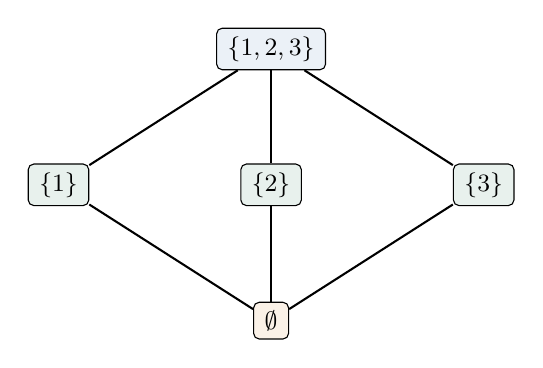
\begin{tikzpicture}[
  x=1.35cm,
  y=1.15cm,
  every node/.style={font=\small},
  flatnode/.style={
    draw,
    rounded corners=2pt,
    inner xsep=4pt,
    inner ysep=3pt,
    fill=white
  },
  edge/.style={line width=0.75pt}
]
  \node[flatnode, fill=pBlue!12] (top) at (0,3) {$\{1,2,3\}$};
  \node[flatnode, fill=pGreen!14] (a) at (-2,1.5) {$\{1\}$};
  \node[flatnode, fill=pGreen!14] (b) at (0,1.5) {$\{2\}$};
  \node[flatnode, fill=pGreen!14] (c) at (2,1.5) {$\{3\}$};
  \node[flatnode, fill=pOrange!13] (bot) at (0,0) {$\emptyset$};

  \draw[edge] (bot) -- (a);
  \draw[edge] (bot) -- (b);
  \draw[edge] (bot) -- (c);
  \draw[edge] (a) -- (top);
  \draw[edge] (b) -- (top);
  \draw[edge] (c) -- (top);
\end{tikzpicture}

\end{document}
